
\documentclass[10pt, a4paper, twocolumn]{article}

\usepackage[english]{babel} % English language hyphenation

\usepackage{microtype} % Better typography

\usepackage{amsmath,amsfonts,amsthm} % Math packages for equations

\usepackage[svgnames]{xcolor} % Enabling colors by their 'svgnames'

\usepackage[hang, small, labelfont=bf, up, textfont=it]{caption} % Custom captions under/above tables and figures

\usepackage{booktabs} % Horizontal rules in tables

\usepackage{lastpage} % Used to determine the number of pages in the document (for "Page X of Total")

\usepackage{graphicx} % Required for adding images

\usepackage{enumitem} % Required for customising lists
\setlist{noitemsep} % Remove spacing between bullet/numbered list elements

\usepackage{sectsty} % Enables custom section titles
\allsectionsfont{\usefont{OT1}{phv}{b}{n}} % Change the font of all section commands (Helvetica)

\usepackage{xcolor}
\usepackage{hyperref}
% https://tex.stackexchange.com/questions/202128/how-to-get-url-and-href-displayed-identically

\hypersetup{colorlinks=true,
linkcolor=black,
urlcolor=gray
% linkcolor=blue,
% urlcolor=blue
}
\urlstyle{rm}

% https://stackoverflow.com/questions/26748820/how-to-change-color-of-hline-in-latex
\usepackage{colortbl}


%----------------------------------------------------------------------------------------
%	MARGINS AND SPACING
%----------------------------------------------------------------------------------------

\usepackage{geometry} % Required for adjusting page dimensions

\geometry{
	top=1cm, % Top margin
	bottom=1.5cm, % Bottom margin
	left=2cm, % Left margin
	right=2cm, % Right margin
	includehead, % Include space for a header
	includefoot, % Include space for a footer
	%showframe, % Uncomment to show how the type block is set on the page
}

\setlength{\columnsep}{7mm} % Column separation width

%----------------------------------------------------------------------------------------
%	FONTS
%----------------------------------------------------------------------------------------

\usepackage[T1]{fontenc} % Output font encoding for international characters
\usepackage[utf8]{inputenc} % Required for inputting international characters

\usepackage{XCharter} % Use the XCharter font

%----------------------------------------------------------------------------------------
%	HEADERS AND FOOTERS
%----------------------------------------------------------------------------------------

\usepackage{fancyhdr} % Needed to define custom headers/footers
\pagestyle{fancy} % Enables the custom headers/footers

\renewcommand{\headrulewidth}{0.0pt} % No header rule
\renewcommand{\footrulewidth}{0.4pt} % Thin footer rule

\renewcommand{\sectionmark}[1]{\markboth{#1}{}} % Removes the section number from the header when \leftmark is used

% \nouppercase\leftmark % Add this to one of the lines below if you want a section title in the header/footer

% Headers
\lhead{} % Left header
\chead{\textit{\thetitle $ $ -- Product Manager}} % Center header - currently printing the article title
\rhead{} % Right header

% Footers
\lfoot{} % Left footer
\cfoot{% % % % %
\href{mailto:venhamon@gmail.com}{venhamon@gmail.com}
|
\href{https://www.linkedin.com/in/bj-pm/}{linkedin.com/in/bj-pm}
|
\href{www.powerinsideout.com}{Coached by powerinsideout.com}
\href{https://www.phyl.org/}{+ NSA}
% Community
| \today
} % Center footer
% \rfoot{\footnotesize
% % Page \thepage\ of \pageref{LastPage}
} % Right footer, "Page 1 of 2"

\fancypagestyle{firstpage}{ % Page style for the first page with the title
	\fancyhf{}
% 	\renewcommand{\footrulewidth}{0pt} % Suppress footer rule
\cfoot{% % % % %
\href{mailto:venhamon@gmail.com}{venhamon@gmail.com}
|
\href{https://www.linkedin.com/in/bj-pm/}{linkedin.com/in/bj-pm}
|
\href{www.powerinsideout.com}{Coached by powerinsideout.com}
\href{https://www.phyl.org/}{+ NSA}
| \today
}
}

%----------------------------------------------------------------------------------------
%	TITLE SECTION
%----------------------------------------------------------------------------------------

\newcommand{\authorstyle}[1]{{\large\usefont{OT1}{phv}{b}{n}\color{DarkRed}#1}} % Authors style (Helvetica)

\newcommand{\institution}[1]{{\footnotesize\usefont{OT1}{phv}{m}{sl}\color{Black}#1}} % Institutions style (Helvetica)

\usepackage{titling} % Allows custom title configuration

\newcommand{\HorRule}{\color{DarkGoldenrod}\rule{\linewidth}{1pt}} % Defines the gold horizontal rule around the title

\pretitle{
	\vspace{-80pt} % Move the entire title section up
	\HorRule\vspace{5pt} % Horizontal rule before the title
	\fontsize{32}{36}\usefont{OT1}{phv}{b}{n}\selectfont % Helvetica
	\color{DarkRed} % Text colour for the title and author(s)
}

\posttitle{\par\vskip 5pt} % Whitespace under the title

\preauthor{} % Anything that will appear before \author is printed

\postauthor{ % Anything that will appear after \author is printed
	\vspace{10pt} % Space before the rule
	\par\HorRule % Horizontal rule after the title
% 	\vspace{0pt} % Space after the title section
}

%----------------------------------------------------------------------------------------
%	ABSTRACT
%----------------------------------------------------------------------------------------

\usepackage{lettrine} % Package to accentuate the first letter of the text (lettrine)
\usepackage{fix-cm}	% Fixes the height of the lettrine

\newcommand{\initial}[1]{ % Defines the command and style for the lettrine
	\lettrine[lines=3,findent=4pt,nindent=0pt]{% Lettrine takes up 3 lines, the text to the right of it is indented 4pt and further indenting of lines 2+ is stopped
		\color{DarkGoldenrod}% Lettrine colour
		{#1}% The letter
	}{}%
}

\usepackage{xstring} % Required for string manipulation

\newcommand{\lettrineabstract}[1]{
	\StrLeft{#1}{1}[\firstletter] % Capture the first letter of the abstract for the lettrine
	\initial{\firstletter}\textbf{\StrGobbleLeft{#1}{1}} % Print the abstract with the first letter as a lettrine and the rest in bold
}

%----------------------------------------------------------------------------------------
%	BIBLIOGRAPHY
%----------------------------------------------------------------------------------------

% \usepackage[backend=bibtex,style=authoryear,natbib=true]{biblatex} % Use the bibtex backend with the authoryear citation style (which resembles APA)
%
% \addbibresource{example.bib} % The filename of the bibliography

% \usepackage[autostyle=true]{csquotes} % Required to generate language-dependent quotes in the bibliography

%%%%%%%%%%%%%%%%%%%%%%%%%%%%%%%%%%%%%%%%%
% Wenneker Article
% Structure Specification File
% Version 1.0 (28/2/17)
%
% This file originates from:
% http://www.LaTeXTemplates.com
%
% Authors:
% Frits Wenneker
% Vel (vel@LaTeXTemplates.com)
%
% License:
% CC BY-NC-SA 3.0 (http://creativecommons.org/licenses/by-nc-sa/3.0/)
%
%%%%%%%%%%%%%%%%%%%%%%%%%%%%%%%%%%%%%%%%%

%----------------------------------------------------------------------------------------
%	PACKAGES AND OTHER DOCUMENT CONFIGURATIONS
%----------------------------------------------------------------------------------------
 % Specifies the document structure and loads requires packages

\title{Benji J} % The article title

\author{
	\authorstyle{Product Manager | SaaS and Mobile App, Music, Web3 } \\ \\
\textbf{Summary} \\
Benji researched in Sociology over a decade.
Between 2021-2022 he's been working as Project Manager, and then Product Manager %@NEWM as the first full time product person to  build % the initial parts of the ecosystem
building with design and development.
He works in small teams to create small impactful launches from ideation to post-launch. % including product review with users and iterating for product-market fit.
Attends to UX flows, copywriting, research, data analytics, strategy and growth.
Likes Web3/Crypto as a needed personal tool for stable coins, and learning about finance and IP rights. \\ \\
\textbf{Career Goals} \\
% % % % % % % % % % % %
\textit{Short-Term (6 months)} \\
Focus on industries:
  Crypto,
  Urban,
  Travel,
  Social-Environmental Impact,
  Cyber Security,
  UX and UI Design \\ \\
% % % % % % % % % % % %
  \textit{Mid-Term (6+ months --- 3 years)} \\
Develop strategy skills, %regardless of role title;
focus on user/s journey, discovery, UX,
positive team impact,
business results, and growth \\ \\
% % % % % % % % % % % %
\textit{Long-Term (5+ years)} \\
Well established profile suitable for creating,
or working closely,
on: vision, mission, new market segments \\ \\
% % % % % % % % % % % %
\textbf{Location preference}     \\
Remote, NYC timezone.
OK travel 3/4 times per year
for
team retreat or offsite. \\ \\
% % % % % % % % % % % %
\textbf{Company stage preference}     \\
Series A
% (Growth: B/C)
} % to do in-office work, or % company offsite or
% % % % % % % % % % % %
% % % % % % % % % % % %

% Example of a one line author/institution relationship
%\author{\newauthor{John Marston} \newinstitution{Universidad Nacional Autónoma de México, Mexico City, Mexico}}

\date{%\today
% \textbf{Summary.}
% Benji has a background in Sociology spanning over a decade. Always aiming for Product work, in 2021 he started working as a Project Manager, and then from 2022 as a Web3/Crypto Product Manager @NEWM as the first full time person to build the initial parts of the ecosystem. His experise is to work in small teams and coordinate small but impactful launches from ideation to post-launch, including product review with users and iterating for product-market fit.
% He aims for extra attention to UX flows, copywriting, research, data analytics, strategy and growth.
}
% Add a date here if you would like one to appear underneath the title block, use \today for the current date, leave empty for no date

%----------------------------------------------------------------------------------------

\begin{document}
% 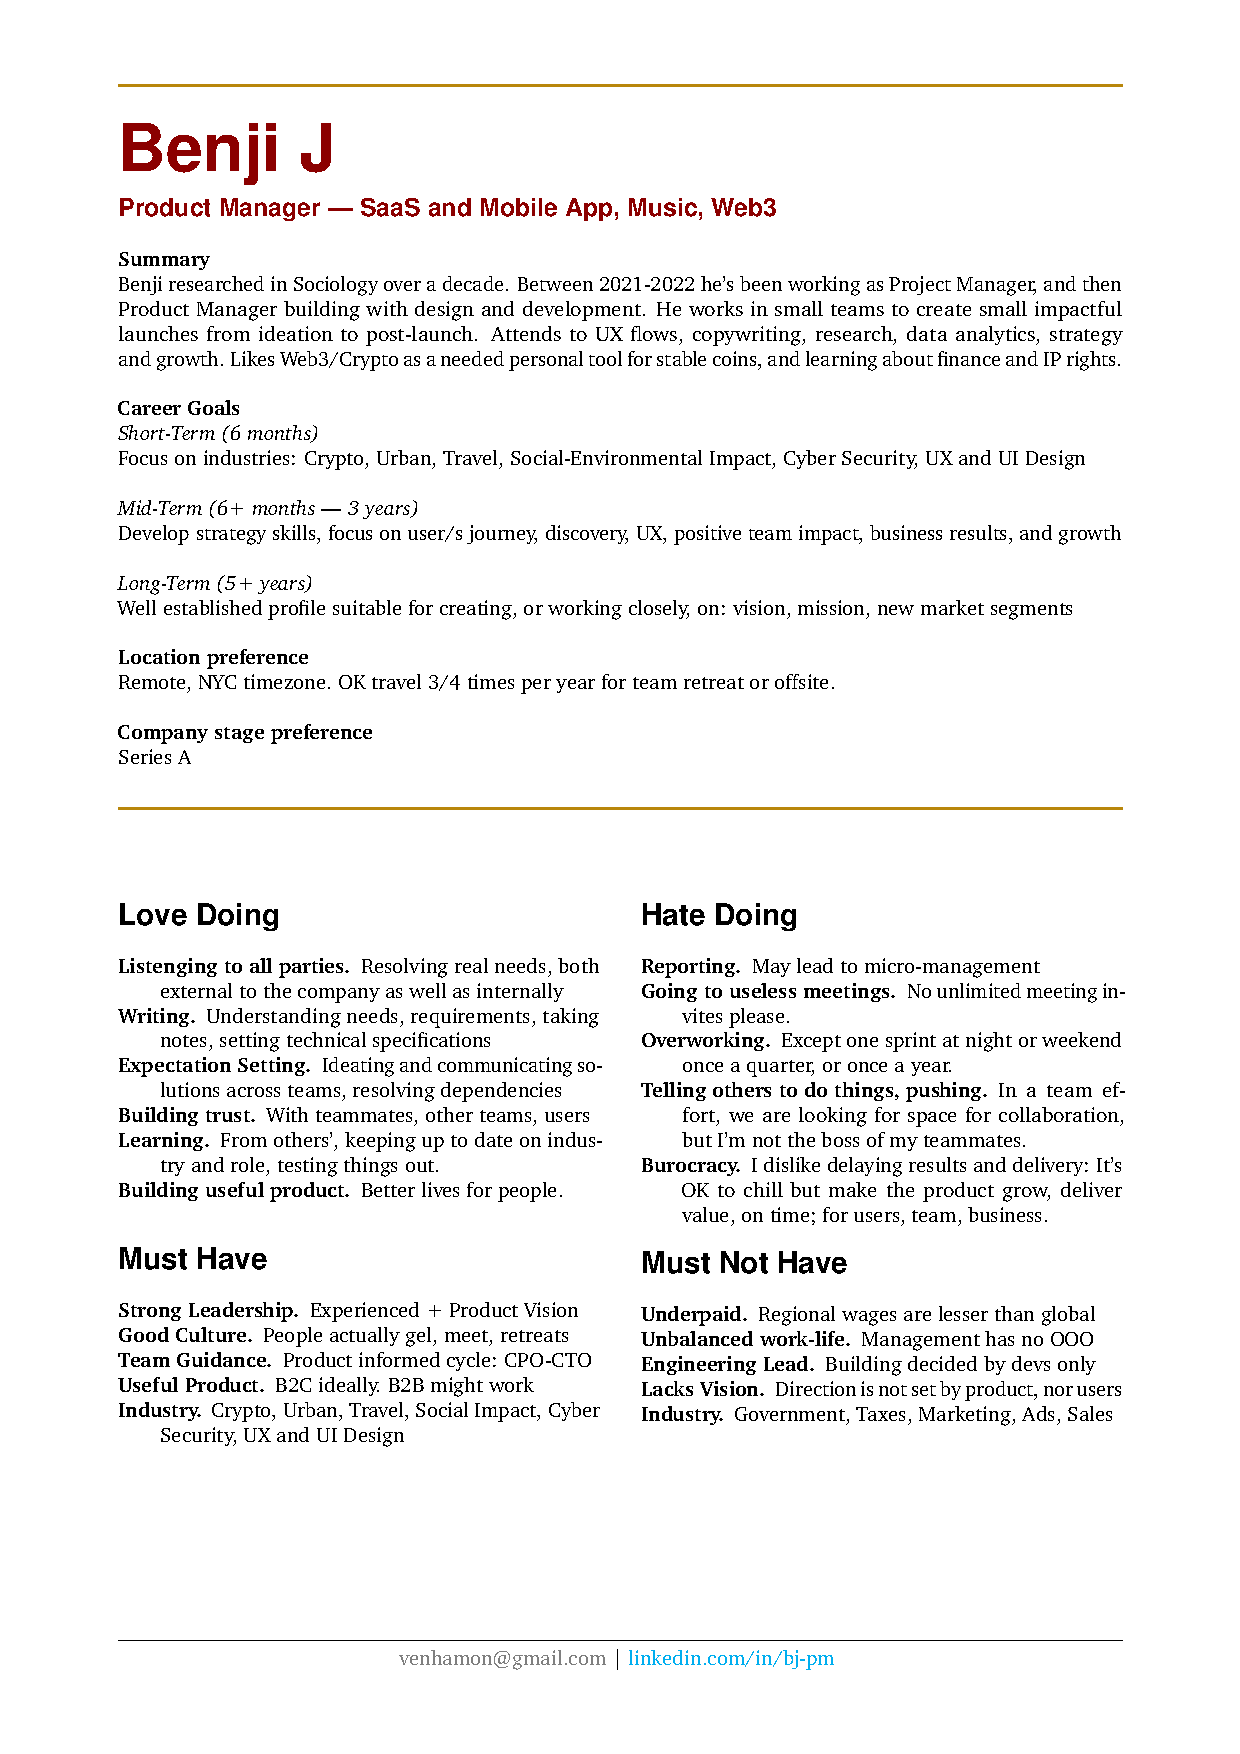
\includepdf[pages={1}]{main.pdf}

\maketitle % Print the title
\thispagestyle{firstpage} % IMPORTANT FOOTER
% \thispagestyle{headings}
% \thispagestyle{empty}
% \thispagestyle{plain}
% Apply the page style for the first page (no headers and footers)
% \vfill\eject


% ----------------------------------------------------------------------------------------
% % 	SUMMARY % ABSTRACT
% ----------------------------------------------------------------------------------------
%
% \section*{Summary}
%
% \lettrineabstract{Benji has a background in Sociology spanning over a decade. %including a Masters degree research in Graffiti and Urban Art, with experience in observing behaviour, taking notes in account for interviews and detail of context.
% % He is an early user of open source software, using Linux from 2005 onwards, also using later on: \LaTeX, vim, git, and always looking for independent sources for creation and production.
% % Since
% % 2019 he's %studying as a Systems Analyst and from the same period has
% % been working in tech in different capacities: backend developer, technical writer, and more recently
% Always aiming for Product work, in 2021 he started working as a Project Manager, and then from 2022 as a Web3/Crypto Product Manager @NEWM as the first full time person to build the initial parts of the ecosystem.
% His experise is to work in small teams and coordinate small but impactful launches from ideation to post-launch, including product review with users and iterating for product-market fit.
% %
% He %has touched all major product components and particularly
% % enjoys being the voice of the customer, with special
% aims for extra
% attention to UX flows, copywriting, research, data analytics, strategy and growth.
% % : a platform for musicians to distribute their music with 100\% ownership and the capability of selling their ability to earn revenue from their royalties;
% % a platform for fans to buy future revenue for royalties;
% % a mobile app to listen to the music distributed,
% }
% % Lorem ipsum dolor sit amet, consectetur adipiscing elit. Fusce maximus nisi ligula. Morbi laoreet ex ligula, vitae lobortis purus mattis vel. Vestibulum ante ipsum primis in faucibus orci luctus et ultrices posuere cubilia Curae; Donec ac metus ut turpis mollis placerat et nec enim. Duis tristique nibh maximus faucibus facilisis. Praesent in consequat leo. Maecenas condimentum ex rhoncus, elementum diam vel, malesuada ante.

% \section*{Summary}

%
% \section*{Career Goals}
%
% \subsection*{Short-Term (3-5 years)}
% \begin{description}
%
% \item[Immediate 6 months:]
%  \item[] yada yada
%  \item[]bla bla bla
% \item[6+ months - 3 years.] \newline
%  \item[] yada yada
%  \item[]bla bla bla
% % Resolving real needs, both external to the company as well as internally
% % \item[Writing.] Understanding needs, requirements, taking notes, setting technical specifications
% % \item[Expectation Setting.] Ideating and communicating solutions across teams, resolving dependencies
% % \item[Useful Product.] B2C ideally. B2B might work
%
% \end{description}
%
%
% \subsection*{Long-Term (5+ years)}
%
% \begin{description}
%
% \item[6+ months - 3 years.] yada yada
% % \item[Writing.] Understanding needs, requirements, taking notes, setting technical specifications
% % \item[Expectation Setting.] Ideating and communicating solutions across teams, resolving dependencies
% % \item[Useful Product.] B2C ideally. B2B might work
%
% \end{description}

% \vfill\eject


\section*{Love Doing}

\begin{description}

\item[Listenging to all parties.] Resolving real needs, both external to the company as well as internally
\item[Writing.] Understanding needs, requirements, taking notes, setting technical specifications
\item[Expectation Setting.] Ideating and communicating solutions across teams, resolving dependencies
\item[Building trust.] With teammates, other teams, users
\item[Learning.]
From others', %experiences and areas, diving into depth of
keeping up to date on industry and role, testing things out.
\item[Building useful product.]
Better lives for people.
% Creating an impact on people’s lives, for the better. %- ideally working for a mission-driven company.

\end{description}


\section*{Must Have}

\begin{description}
 \item[Strong Leadership.] Experienced + Product Vision
%  Or less Experienced but with Drive and a compelling Roadmap
 \item[Good Culture.] People actually gel, meet, retreats %  Great Place to Work is amazing
  \item[Team Guidance.] Product informed cycle: CPO-CTO
 \item[Useful Product.] B2C ideally. B2B might work
  \item[Industry.]
  Crypto,
  Urban,
  Travel,
  Social Impact,
  Cyber Security,
  UX and UI Design
%   Creative,
%   Entertainment,
%   Health,
\end{description}

% \end{document}







% This sentence requires citation \citep{Reference1}. This sentence requires multiple citations to imply that it is better supported \citep{Reference2,Reference3}. Finally, when conducting an appeal to authority, it can be useful to cite a reference in-text, much like \cite{Reference1} do quite a bit. Oh, and make sure to check out the bear in Figure \ref{bear}.

% \onecolumn

% \vfill\eject

% \end{twocolumn}
%
% \begin{twocolumn}


% \section*{Not Good}
%
%
% Lorem ipsum dolor sit amet, consectetur adipiscing elit. Fusce maximus nisi ligula. Morbi laoreet ex ligula, vitae lobortis purus mattis vel. Vestibulum ante ipsum primis in faucibus orci luctus et ultrices posuere cubilia Curae; Donec ac metus ut turpis mollis placerat et nec enim. Duis tristique nibh maximus faucibus facilisis. Praesent in consequat leo. Maecenas condimentum ex rhoncus, elementum diam vel, malesuada ante. Fusce pulvinar, mauris pretium placerat venenatis, lectus ex tempus lacus, id suscipit libero lorem eu augue. Interdum et malesuada fames ac ante ipsum primis in faucibus.
%

\vfill\eject

\section*{Hate Doing}

\begin{description}
 \item[Reporting.] May lead to micro-management
 \item[Going to useless meetings.] No unlimited meeting invites please.
 \item[Overworking.] Except one sprint at night or weekend once a quarter, or once a year.
 \item[Telling others to do things, pushing.] In a team effort, we are looking for space for collaboration, but I'm not the boss of my teammates.
  \item[Burocracy.] I dislike delaying results and delivery:
% You need to lay back a bit,
 It's OK to chill
 but %also
 make the product grow, deliver value, on time;
 for users, team, business.
%  \item[]
\end{description}

% \smallskip

  \vspace*{-20pt}

\section*{Must Not Have}

\begin{description}
 \item[Underpaid.] Regional wages are lesser than global
  \item[Unbalanced work-life.] Management has no OOO
    \item[Engineering Lead.] Building decided by devs only
 \item[Lacks Vision.] Direction is not set by product, nor users
  \item[Industry.] Government, Taxes, Marketing, Ads, Sales
%  \item[Good Culture.] People actually gel, meet, retreats %  Great Place to Work is amazing
%  \item[Useful Product.] B2C ideally. B2B might work
%   \item[Industry.]
%   Crypto,
%   Urban,
%   Travel,
%   Social Impact
%   Creative,
%   Entertainment,
%   Health,
\end{description}


% This sentence requires citation \citep{Reference1}. This sentence requires multiple citations to imply that it is better supported \citep{Reference2,Reference3}. Finally, when conducting an appeal to authority, it can be useful to cite a reference in-text, much like \cite{Reference1} do quite a bit. Oh, and make sure to check out the bear in Figure \ref{bear}.

% \end{document}


% \section*{Personality}
%
% \subsection*{Myers Briggs}
% \begin{description}
%
% %  \item[INTJ: Architect.] Architects are imaginative and strategic thinkers, with a plan for everything.
%  \item[INTJ: Architect] %Architects are
%  \item[] Imaginative + Strategy / Planning
% %  thinkers, with a plan for everything.
% \end{description}
%
%
%  \subsection*{Enneagram}
%  \begin{description}
%
%  \item[Type 5 / Wing 4 -- The Iconoclast] %\newline
%  \item[] creativeness + sensitivity
% %  is a subtype that results from the encounter of types 5 and 4, which means that the sensitivity of the 4s is added to the natural creativeness of 5s.
%  \end{description}

%  -%Architects are imaginative and strategic thinkers, with a plan for everything.


% \end{document}


\clearpage

\section*{Strengths \& Weaknesses}

\subsection*{Strengths}

\begin{description}
 \item[Belief] in: self, others, team, company. My view of the compant and team make me super high drive, and persistent.
\item[Curious.] I love learning, but my fuel is in placing questions forward and not staying stagnant with a simple eternal answer. Iteration and nuance are key.
\item[Supportive.] I push causes to happen, and I believe we can all give something out to the world. wagmi: we're all gonna make it.
\item[Ownership.] I believe to have both confidence and certainty to move forward, and I strive for other people to gain them as well.
\item[Strategist.] Always aiming for the big picture: am I going to be happy about this work in 20 to 50/200 years? I truly hope so.
 \end{description}

\subsection*{Weaknesses}

\begin{description}
 \item[Contrarian:] sometimes wrongly
 \item[Interruptor:] a fine art that should never be learned
 \item[Overly Imaginative:] going off rail to derivatives can be unproductive for working on immediate goals. Let's better plan one step at a time %so we can
 to stay in sync
 \item[Unexperienced Professional Background:]
no well-known, big-name company on my resume as an employer.
Primary experience in unstructured companies, mostly regional, in LatinAmerica, and in a promising Music Startup (with HQ in US and Europe) but that hasn't yet gained traction.
%  \item[]
%  \item[]
 \end{description}

% \section*{Must Have}
%
% \begin{description}
%  \item[Strong Leadership.] Experienced + Product Vision
% %  Or less Experienced but with Drive and a compelling Roadmap
%  \item[Good Culture.] People actually gel, meet, retreats %  Great Place to Work is amazing
%   \item[Team Guidance.] Product informed cycle: CPO-CTO
%  \item[Useful Product.] B2C ideally. B2B might work
%   \item[Industry.]
%   Crypto,
%   Urban,
%   Travel,
%   Social Impact, Cyber Security, UX and UI Design
% %   Creative,
% %   Entertainment,
% %   Health,
% \end{description}

\vfill\eject


\section*{Personality}

\subsection*{Gallup Strengths}
\begin{description}
 \item [Believer]
 \item [Philomath]
 \item [Coach]
 \item [Self-Believer]
 \item [Strategist]
\end{description}



\subsection*{Myers Briggs}
\begin{description}

%  \item[INTJ: Architect.] Architects are imaginative and strategic thinkers, with a plan for everything.
 \item[INTJ: Architect] %Architects are
 \item[] Imaginative + Strategy / Planning
%  thinkers, with a plan for everything.
\end{description}


 \subsection*{Enneagram}
 \begin{description}

 \item[Type 5 / Wing 4 -- The Iconoclast] %\newline
 \item[] creativeness + sensitivity
%  is a subtype that results from the encounter of types 5 and 4, which means that the sensitivity of the 4s is added to the natural creativeness of 5s.
 \end{description}

%  -%Architects are imaginative and strategic thinkers, with a plan for everything.

\section*{Candidate-Market Fit}
% Seeking a Product Manager remote role with attention to Growth and UX at a SaaS-based tech company, ideally B2C but comfortable with B2B.
% Growth
\textit{%
Seeking a Product Manager remote role
with attention to UX
at a Series-A SaaS-based tech company in Crypto,
ideally with social impact and/or B2C.
}
\\ \\
My background is in sociology and systems analysis. I enjoy user feedback roles, discovery and beta testing.
% Prefer a role that includes other Product Manager, or near: above or below.
% Interested in joining a start-up in an in-demand industry. % % % % % % % % %
% If given a choice, my
\subsection*{Preferred industries}
\begin{description}
 \item Crypto
\item Urban
\item Travel
\item Social Impact
\item Cyber Security
\item UX and UI Design
\item Publishing and Entertainment
\item Gaming
\item Ed Tech
\end{description}
% \\ \\
% I am open to other opportunities as I do not have direct industry experience in these fields.
% My background is in sociology and systems analysis. I enjoy user feedback roles, discovery and beta testing.


% This sentence requires citation \citep{Reference1}. This sentence requires multiple citations to imply that it is better supported \citep{Reference2,Reference3}. Finally, when conducting an appeal to authority, it can be useful to cite a reference in-text, much like \cite{Reference1} do quite a bit. Oh, and make sure to check out the bear in Figure \ref{bear}.

% \onecolumn

\vfill\eject

% \end{twocolumn}
%
% \begin{twocolumn}


% \section*{Not Good}
%
%
% Lorem ipsum dolor sit amet, consectetur adipiscing elit. Fusce maximus nisi ligula. Morbi laoreet ex ligula, vitae lobortis purus mattis vel. Vestibulum ante ipsum primis in faucibus orci luctus et ultrices posuere cubilia Curae; Donec ac metus ut turpis mollis placerat et nec enim. Duis tristique nibh maximus faucibus facilisis. Praesent in consequat leo. Maecenas condimentum ex rhoncus, elementum diam vel, malesuada ante. Fusce pulvinar, mauris pretium placerat venenatis, lectus ex tempus lacus, id suscipit libero lorem eu augue. Interdum et malesuada fames ac ante ipsum primis in faucibus.
%
% \vfill\eject
%
% \section*{Hate}
%
% \begin{description}
%  \item[Underpaid.] Regional wages are lesser than global
%   \item[Unbalanced work-life.] Management has no OOO
%     \item[Engineering Lead.] Building decided by devs only
%  \item[Lacks Vision.] Direction is not set by product, nor users
%   \item[Industry.] Government, Taxes, Marketing, Ads, Sales
% %  \item[Good Culture.] People actually gel, meet, retreats %  Great Place to Work is amazing
% %  \item[Useful Product.] B2C ideally. B2B might work
% %   \item[Industry.]
% %   Crypto,
% %   Urban,
% %   Travel,
% %   Social Impact
% %   Creative,
% %   Entertainment,
% %   Health,
% \end{description}
%
% \smallskip
%
% \section*{Must Not Have}
%
% \begin{description}
%  \item[Underpaid.] Regional wages are lesser than global
%   \item[Unbalanced work-life.] Management has no OOO
%     \item[Engineering Lead.] Building decided by devs only
%  \item[Lacks Vision.] Direction is not set by product, nor users
%   \item[Industry.] Government, Taxes, Marketing, Ads, Sales
% %  \item[Good Culture.] People actually gel, meet, retreats %  Great Place to Work is amazing
% %  \item[Useful Product.] B2C ideally. B2B might work
% %   \item[Industry.]
% %   Crypto,
% %   Urban,
% %   Travel,
% %   Social Impact
% %   Creative,
% %   Entertainment,
% %   Health,
% \end{description}



\end{document}

%%%%%%%%%%%%%%%%%%%%%%%%%%%%%%%%%%%%%%%%%
% Wenneker Article
% LaTeX Template
% Version 2.0 (28/2/17)
%
% This template was downloaded from:
% http://www.LaTeXTemplates.com
%
% Authors:
% Vel (vel@LaTeXTemplates.com)
% Frits Wenneker
%
% License:
% CC BY-NC-SA 3.0 (http://creativecommons.org/licenses/by-nc-sa/3.0/)
%
%%%%%%%%%%%%%%%%%%%%%%%%%%%%%%%%%%%%%%%%%

%----------------------------------------------------------------------------------------
%	PACKAGES AND OTHER DOCUMENT CONFIGURATIONS
%----------------------------------------------------------------------------------------


%----------------------------------------------------------------------------------------
%	ABSTRACT
%----------------------------------------------------------------------------------------

% \lettrineabstract{Lorem ipsum dolor sit amet, consectetur adipiscing elit. Fusce maximus nisi ligula. Morbi laoreet ex ligula, vitae lobortis purus mattis vel. Vestibulum ante ipsum primis in faucibus orci luctus et ultrices posuere cubilia Curae; Donec ac metus ut turpis mollis placerat et nec enim. Duis tristique nibh maximus faucibus facilisis. Praesent in consequat leo. Maecenas condimentum ex rhoncus, elementum diam vel, malesuada ante.}

%----------------------------------------------------------------------------------------
%	ARTICLE CONTENTS
%----------------------------------------------------------------------------------------

% \section*{Good}
%
% \begin{description}
%  \item[Strong Leadership.] Experienced + Product Vision
% %  Or less Experienced but with Drive and a compelling Roadmap
%  \item[Good Culture.] People actually gel, meet, retreats %  Great Place to Work is amazing
%  \item[Useful Product.] B2C ideally. B2B might work
%   \item[Industry.] Entertainment, Creative, Travel, Health
% \end{description}

% This sentence requires citation \citep{Reference1}. This sentence requires multiple citations to imply that it is better supported \citep{Reference2,Reference3}. Finally, when conducting an appeal to authority, it can be useful to cite a reference in-text, much like \cite{Reference1} do quite a bit. Oh, and make sure to check out the bear in Figure \ref{bear}.


% % % % % % % % % % % % % % % % %

% 10pt font size (11 and 12 also possible), A4 paper (letterpaper for US letter) and two column layout (remove for one column)
% \usepackage[1]{pagesel}
% https://tex.stackexchange.com/questions/96256/compiling-only-a-page-range-or-page-selection
